\documentclass[11pt,a4paper]{article}
% ---------------------------------------------------------------
% Preamble — biên dịch bằng XeLaTeX (tectonic)
% ---------------------------------------------------------------
\usepackage{fontspec}
\usepackage{unicode-math}

% Font chính: CM Unicode (phủ đủ dấu tiếng Việt). Nếu không có, đổi sang
% \setmainfont{Times New Roman} hoặc \setmainfont{Arial Unicode}.
\IfFontExistsTF{cmunrm.otf}{%
  \setmainfont{cmun}[
    Extension      = .otf,
    UprightFont    = *rm,
    BoldFont       = *bx,
    ItalicFont     = *ti,
    BoldItalicFont = *bi,
    Ligatures      = TeX ]
  \setmonofont{cmun}[
    Extension      = .otf,
    UprightFont    = *tt,
    BoldFont       = *tb,
    ItalicFont     = *it,
    Scale          = 0.92 ]
}{%
  \setmainfont{Times New Roman}[Ligatures=TeX]
  \setmonofont{Menlo}[Scale=0.85]
}

\usepackage[a4paper,top=2.5cm,bottom=2.5cm,left=2.6cm,right=2.6cm]{geometry}
\usepackage{amsmath}
\usepackage{graphicx}
\usepackage{float}
\usepackage{xcolor}
\usepackage{booktabs}
\usepackage{longtable}
\usepackage{tabularx}
\usepackage{array}
\usepackage{multirow}
\usepackage{enumitem}
\usepackage{caption}
\usepackage{subcaption}
\usepackage{listings}
\usepackage{fancyvrb}
\usepackage{fvextra}
\usepackage{fancyhdr}
\usepackage{titlesec}
\usepackage[most]{tcolorbox}
\usepackage[hidelinks,bookmarksnumbered]{hyperref}

% --------------------------- màu sắc ---------------------------
\definecolor{accent}{HTML}{1F4E79}
\definecolor{softbg}{HTML}{F3F6FA}
\definecolor{softbd}{HTML}{9DB8D4}
\definecolor{warmbg}{HTML}{FDF2E3}
\definecolor{warmbd}{HTML}{E0A458}
\definecolor{coolbg}{HTML}{EAF5EF}
\definecolor{coolbd}{HTML}{5CA184}
\definecolor{rulegray}{HTML}{BBBBBB}
\definecolor{codebg}{HTML}{F7F7F7}

% --------------------------- tiêu đề ---------------------------
\titleformat{\section}{\Large\bfseries\color{accent}}{\thesection.}{0.5em}{}
\titleformat{\subsection}{\large\bfseries}{\thesubsection}{0.5em}{}
\titlespacing*{\section}{0pt}{1.4em}{0.7em}
\titlespacing*{\subsection}{0pt}{1.1em}{0.5em}

\pagestyle{fancy}
\fancyhf{}
\fancyfoot[C]{\small\thepage}
\renewcommand{\headrulewidth}{0pt}

% --------------------------- bảng ------------------------------
\newcolumntype{L}[1]{>{\raggedright\arraybackslash}p{#1}}
\newcolumntype{C}[1]{>{\centering\arraybackslash}p{#1}}
\newcolumntype{R}[1]{>{\raggedleft\arraybackslash}p{#1}}
\newcolumntype{Y}{>{\raggedright\arraybackslash}X}
\renewcommand{\arraystretch}{1.18}
\captionsetup[table]{font=small,labelfont=bf,skip=4pt}
\captionsetup[figure]{font=small,labelfont=bf,skip=4pt}
\renewcommand{\tablename}{Bảng}
\renewcommand{\figurename}{Hình}
\renewcommand{\contentsname}{Mục lục}

% --------------------------- hộp nhấn mạnh ---------------------
\newtcolorbox{softbox}[1][]{
  colback=softbg, colframe=softbd, boxrule=0.6pt, arc=2pt,
  left=8pt, right=8pt, top=6pt, bottom=6pt, #1}
\newtcolorbox{warmbox}[1][]{
  colback=warmbg, colframe=warmbd, boxrule=0.6pt, arc=2pt,
  left=8pt, right=8pt, top=6pt, bottom=6pt, #1}
\newtcolorbox{coolbox}[1][]{
  colback=coolbg, colframe=coolbd, boxrule=0.6pt, arc=2pt,
  left=8pt, right=8pt, top=6pt, bottom=6pt, #1}
\newtcolorbox{plainbox}[1][]{
  colback=white, colframe=black, boxrule=0.5pt, arc=1pt,
  left=8pt, right=8pt, top=6pt, bottom=6pt, #1}

% --------------------------- code ------------------------------
\lstdefinestyle{plain}{
  basicstyle=\ttfamily\scriptsize,
  breaklines=true,
  breakatwhitespace=false,
  columns=fullflexible,
  keepspaces=true,
  showstringspaces=false,
  backgroundcolor=\color{codebg},
  frame=single,
  rulecolor=\color{rulegray},
  framesep=4pt,
  xleftmargin=6pt,
  xrightmargin=2pt,
  numbers=none,
  upquote=true,
  extendedchars=true,
  % Không dùng `literate`: XeTeX xử lý UTF-8 trực tiếp, cmuntt phủ đủ dấu tiếng Việt.
}
\lstset{style=plain}

% listings không xử lý đúng ký tự UTF-8 3 byte (ộ, ữ, ệ...). Mọi tệp mã nguồn
% có tiếng Việt được nạp bằng fvextra/fancyvrb — XeTeX đọc UTF-8 trực tiếp.
\newcommand{\srcfile}[2][]{%
  \VerbatimInput[fontsize=\scriptsize, frame=single, framesep=4pt,
    rulecolor=\color{rulegray}, breaklines, breakanywhere,
    breaksymbolleft={}, breaksymbolright={}, #1]{#2}}

% --------------------------- tiện ích --------------------------
\newcommand{\kpi}[2]{%
  \begin{minipage}[t]{0.24\linewidth}\centering
    {\large\bfseries #1}\\[2pt]{\footnotesize #2}
  \end{minipage}}
\newcommand{\req}{\textsuperscript{\textcolor{accent}{\scriptsize[BẮT BUỘC]}}}
\setlist[itemize]{leftmargin=1.4em,itemsep=2pt,topsep=3pt}
\setlist[enumerate]{leftmargin=1.7em,itemsep=2pt,topsep=3pt}

% --------------------------- bổ sung cho A4–A5 --------------------
\usepackage{multirow}
\usepackage{pdflscape}
\newcommand{\code}[1]{\texttt{\small #1}}
% Bảng dài dùng chung một kiểu chữ nhỏ
\newcommand{\smalltable}{\small}

% --------------------------- bổ sung cho A7 --------------------
\usepackage{tikz}
\usetikzlibrary{arrows.meta,positioning,fit,calc,backgrounds}
\tikzset{
  op/.style={draw, rounded corners=2pt, minimum height=5.5mm, minimum width=9mm,
             font=\scriptsize\ttfamily, fill=white},
  var/.style={font=\small, inner sep=1pt},
  flow/.style={-{Stealth[length=4pt]}, semithick},
}
\definecolor{rnncol}{HTML}{C8553D}
\definecolor{lstmcol}{HTML}{2E6F95}

\usepackage{tikz}
\usetikzlibrary{arrows.meta,positioning,fit,calc}
\newcommand{\nDocs}{35}
\newcommand{\nDocsVi}{13}
\newcommand{\nDocsEn}{22}
\newcommand{\nHtmlVi}{10}
\newcommand{\nHtmlEn}{18}
\newcommand{\nPdfVi}{3}
\newcommand{\nPdfEn}{4}
\newcommand{\nPublishers}{16}
\newcommand{\nChunks}{424}
\newcommand{\nChunksVi}{273}
\newcommand{\nChunksEn}{151}
\newcommand{\tokMean}{337}
\newcommand{\tokMin}{63}
\newcommand{\tokMax}{400}
\newcommand{\nQuestions}{30}
\newcommand{\nInScope}{26}
\newcommand{\nOos}{4}
\newcommand{\nQEn}{4}
\newcommand{\nGoldPairs}{269}
\newcommand{\goldMin}{2}
\newcommand{\goldMax}{21}
\newcommand{\poolMean}{48}
\newcommand{\relAgree}{12/15}
\newcommand{\relAgreeLenient}{15--17/25}
\newcommand{\claimAgree}{5/5}
\newcommand{\nFacts}{1.779}
\newcommand{\nBilingualFacts}{52}
\newcommand{\nProposed}{2.195}
\newcommand{\nAccepted}{2.124}
\newcommand{\nRejQuote}{60}
\newcommand{\nRejOther}{11}
\newcommand{\extractTokens}{522.949}
\newcommand{\nNodes}{2.846}
\newcommand{\nRels}{5.027}
\newcommand{\nSupportedBy}{2.116}
\newcommand{\nRowsStatus}{686.019}
\newcommand{\nProfilesStatus}{634.636}
\newcommand{\nRowsType}{22.027}
\newcommand{\nFeatures}{19}
\newcommand{\trainSeconds}{66}
\newcommand{\predictMs}{0,033}
\newcommand{\tempStatus}{0,819}
\newcommand{\tempType}{0,612}
\newcommand{\eceStatusBefore}{0,1116}
\newcommand{\eceStatusAfter}{0,0881}
\newcommand{\eceTypeBefore}{0,0962}
\newcommand{\eceTypeAfter}{0,0425}
\newcommand{\eceStatusPrior}{0,0056}
\newcommand{\eceTypePrior}{0,0237}
\newcommand{\bestEpochStatus}{5}
\newcommand{\epochsStatus}{13}
\newcommand{\bestEpochType}{11}
\newcommand{\epochsType}{19}
\newcommand{\preTP}{524}
\newcommand{\preSupport}{2.295}
\newcommand{\prePrecision}{0,0357}
\newcommand{\typeOneTP}{149}
\newcommand{\typeOneSupport}{298}
\newcommand{\typeOnePred}{875}
\newcommand{\typeOnePrecision}{0,1703}
\newcommand{\answeredZero}{24/26}
\newcommand{\answeredTwo}{25/26}
\newcommand{\supportedZero}{98,9\%}
\newcommand{\supportedTwo}{97,9\%}
\newcommand{\unsupportedZero}{0,6\%}
\newcommand{\unsupportedTwo}{0,0\%}
\newcommand{\claimsZero}{175}
\newcommand{\claimsTwo}{186}
\newcommand{\refusalOos}{100\%}
\newcommand{\falseRefusalTwo}{3,9\%}
\newcommand{\falseRefusalZero}{7,7\%}
\newcommand{\latencyP}{2,46}
\newcommand{\latencyMax}{8,82}
\newcommand{\vZeroUnsupported}{39,1\%}
\newcommand{\vOneUnsupported}{4,0\%}
\newcommand{\vOneFalseRefusal}{19,2\%}
\newcommand{\gxAdded}{51}
\newcommand{\gxRelevant}{17,6\%}
\newcommand{\gxOther}{39,2\%}
\newcommand{\gxOutside}{96,1\%}
\newcommand{\gxNew}{7}
\newcommand{\llmModel}{gemma-4}
\newcommand{\uiFirstTextP}{2,9}
\newcommand{\rrfK}{60}
\newcommand{\expandN}{2}
\newcommand{\oosMin}{0,78}
\newcommand{\embedDim}{1.024}
\newcommand{\nPrevalenceOther}{361.959}
\newcommand{\yFifteencA}{213.703}
\newcommand{\yFifteencB}{4.631}
\newcommand{\yFifteencC}{35.346}
\newcommand{\yFifteentotal}{253.680}
\newcommand{\yTwentyThreecA}{361.959}
\newcommand{\yTwentyThreecB}{10.594}
\newcommand{\yTwentyThreecC}{59.786}
\newcommand{\yTwentyThreetotal}{432.339}
\newcommand{\typeCountB}{1.958}
\newcommand{\typeCountC}{20.069}

\makeatletter
\newcommand{\tablerows}[1]{\@@input #1 }
\makeatother

\hypersetup{
  pdftitle={Assignment 08 — Neo4j và RAG tra cứu thông tin đái tháo đường},
  pdfauthor={Trần Xuân Thành}}

\tikzset{
  box/.style={draw=softbd, fill=softbg, rounded corners=2pt, align=center, font=\footnotesize,
              minimum height=1.05cm, text width=3.3cm},
  node/.style={draw=accent, fill=white, rounded corners=2pt, align=center, font=\footnotesize,
               minimum height=0.8cm, text width=2.5cm},
  arr/.style={-{Stealth[length=2mm]}, draw=accent!80!black},
  lab/.style={font=\scriptsize\ttfamily, fill=white, inner sep=1pt}}

\begin{document}

% ==================================================================
\thispagestyle{empty}
\begin{center}
  \vspace*{1.2cm}
  {\large\scshape Học viện Công nghệ Bưu chính Viễn thông}\\[4pt]
  {\normalsize Khoa Công nghệ Thông tin}\\[10pt]
  \rule{0.35\linewidth}{0.4pt}\\[16pt]

  {\normalsize Intelligent System Development — Assignment 08}\\[26pt]

  {\Huge\bfseries Neo4j và RAG}\\[10pt]
  {\large trong tra cứu thông tin về đái tháo đường}\\[36pt]

  {\large\bfseries Trần Xuân Thành}\\[6pt]
  {\small Mã sinh viên: B23DCAT280 \quad·\quad Lớp: E23CNPM01 \quad·\quad Nhóm: 02}\\[4pt]
  {\small Giảng viên hướng dẫn: Dinh Que Tran, Ph.D., Assoc. Prof.}\\[24pt]

  {\small Học kỳ I.2026}
\end{center}

\vspace{0.8cm}
\begin{center}\bfseries Tóm tắt\end{center}
\begin{quote}\small
Bài làm xây dựng một ứng dụng web hỏi đáp về đái tháo đường. Tri thức được thu thập từ
\nDocs{} tài liệu công khai của \nPublishers{} đơn vị xuất bản (\nDocsVi{} tiếng Việt, \nDocsEn{} tiếng Anh),
chia thành \nChunks{} đoạn văn và tổ chức thành đồ thị tri thức \texttt{KB\_diabet} trên Neo4j.
Đồ thị gồm \nNodes{} nút và \nRels{} quan hệ, trong đó \nFacts{} mục dữ kiện y tế (triệu chứng, biến chứng,
yếu tố nguy cơ, khuyến nghị, nhóm thuốc) đều nối về đúng đoạn văn chứa câu trích làm bằng chứng.
Phần hỏi đáp dùng kỹ thuật RAG: tìm đoạn văn liên quan, gửi kèm câu hỏi cho mô hình ngôn ngữ, rồi kiểm tra
trích dẫn trước khi hiển thị. Trên bộ \nQuestions{} câu kiểm tra, hệ thống trả lời \answeredTwo{} câu trong phạm vi,
\supportedTwo{} phát biểu được nguồn trích dẫn hỗ trợ và từ chối đúng \refusalOos{} câu ngoài phạm vi.
Phần phân loại huấn luyện mạng MLP trên \nRowsStatus{} bản ghi khảo sát BRFSS 2015 và 2023;
nhãn dự đoán được dùng để chọn chủ đề tra cứu, không dùng để chẩn đoán.
\end{quote}

\newpage
\tableofcontents
\newpage

% ==================================================================
\section{Giới thiệu}

\subsection{Mục tiêu và phạm vi}

\paragraph{Bài toán.}
Người bệnh và người nhà thường tìm thông tin về đái tháo đường trên mạng. Nguồn tin nhiều, chất lượng không
đều, và một câu khuyến nghị bị tách khỏi điều kiện áp dụng của nó có thể gây hiểu sai. Bài làm đặt ra yêu cầu
cho hệ thống tra cứu như sau: \emph{mọi ý trong câu trả lời phải chỉ được về một đoạn văn cụ thể trong một tài liệu
cụ thể}, và khi kho tài liệu không có thông tin thì hệ thống phải nói rõ là không có, thay vì đoán.

Để đáp ứng yêu cầu đó, bài làm kết hợp ba thành phần:
\begin{itemize}
  \item \textbf{Đồ thị tri thức trên Neo4j.} Neo4j là hệ quản trị cơ sở dữ liệu đồ thị: dữ liệu được lưu thành
        nút (đối tượng) và quan hệ có hướng giữa các nút. Bệnh, triệu chứng, khuyến nghị, đoạn văn và tài liệu đều
        là nút; câu “khuyến nghị này được đoạn văn kia hỗ trợ” là một quan hệ.
  \item \textbf{RAG} (Retrieval-Augmented Generation, sinh câu trả lời có truy xuất). Thay vì để mô hình ngôn ngữ
        trả lời từ trí nhớ, chương trình tìm các đoạn văn liên quan trước, rồi yêu cầu mô hình chỉ dùng các đoạn đó.
  \item \textbf{Bộ phân loại khảo sát.} Một mạng nơ-ron nhiều lớp (MLP) dự đoán nhóm tình trạng từ câu trả lời khảo
        sát sức khỏe; nhãn dự đoán dẫn người dùng tới chủ đề tra cứu phù hợp.
\end{itemize}

\subsection{Kết quả chính}

\begin{center}
\kpi{\answeredTwo}{câu trong phạm vi được trả lời}
\kpi{\supportedTwo}{phát biểu được nguồn hỗ trợ}
\kpi{\refusalOos}{câu ngoài phạm vi bị từ chối}
\kpi{\latencyP{} s}{trung vị thời gian một câu}
\end{center}

\begin{table}[H]
\centering
\caption{Các chức năng của hệ thống và cách thực hiện}
\begin{tabularx}{\linewidth}{L{3.3cm}Y}
\toprule
Chức năng & Cách thực hiện \\
\midrule
Thu thập tri thức & Tải trang web và PDF, trích văn bản, lọc menu và quảng cáo, chia đoạn. \\
Tổ chức tri thức & Lưu tài liệu, đoạn văn và dữ kiện y tế trên Neo4j; mỗi dữ kiện có quan hệ \texttt{SUPPORTED\_BY} tới đoạn chứa câu trích. \\
Hỏi đáp & Tìm đoạn gần nghĩa bằng vector, mở rộng qua đồ thị, mô hình \texttt{\llmModel} viết câu trả lời có trích dẫn, chương trình kiểm trích dẫn. \\
Phân loại và tra cứu & MLP dự đoán nhóm từ \nFeatures{} câu trả lời khảo sát; bảng chủ đề chuyển nhãn thành chủ đề tra cứu. \\
Giao diện web & Ứng dụng Next.js dựng lại từ dự án P-185: trang hỏi đáp, trang đồ thị, trang phân loại. \\
\bottomrule
\end{tabularx}
\end{table}

\begin{warmbox}
Hệ thống là công cụ tra cứu thông tin tham khảo. Nhãn của bộ phân loại dựa trên câu trả lời tự báo cáo,
không phải kết quả xét nghiệm, và không được dùng để chẩn đoán hay chỉ định điều trị cho một người cụ thể.
Mỗi câu trả lời trên giao diện đều kèm lời nhắc này.
\end{warmbox}

% ==================================================================
\section{Dữ liệu}

\subsection{Nguồn tri thức y tế}

\paragraph{Đơn vị xuất bản.}
Kho gồm \nDocs{} tài liệu: \nHtmlVi{} trang web và \nPdfVi{} PDF tiếng Việt, \nHtmlEn{} trang web và \nPdfEn{} PDF
tiếng Anh. Nguồn tiếng Việt gồm ba hướng dẫn chẩn đoán và điều trị của Bộ Y tế (đái tháo đường típ 2,
tiền đái tháo đường, đái tháo đường típ 1 ở trẻ em), trang của các bệnh viện và Viện Dinh dưỡng Quốc gia.
Nguồn tiếng Anh gồm NIDDK (viện nghiên cứu tiểu đường, tiêu hóa và thận của Hoa Kỳ), WHO, NHS (Anh),
NDSS (Úc), MedlinePlus, Diabetes UK, Hiệp hội Đái tháo đường Hoa Kỳ và Bộ Y tế Hồng Kông.

\begin{table}[H]
\centering
\caption{Số tài liệu theo đơn vị xuất bản}
\begin{tabular}{lr}
\toprule
Đơn vị xuất bản & Tài liệu \\
\midrule
\tablerows{generated/table_sources.tex}
\bottomrule
\end{tabular}
\end{table}

\paragraph{Nguồn không đưa vào được.}
Các trang của CDC (Hoa Kỳ) trả mã lỗi 403 cho chương trình tải tự động; bài làm tôn trọng lệnh chặn này và không
đưa CDC vào kho. Đường dẫn gốc của các quyết định Bộ Y tế trên cổng kcb.vn trả lỗi 404, nên văn bản được lấy từ
bản đăng lại trên website bệnh viện, cùng số quyết định. Một trang giải thích HbA1c bị loại vì ghi nhầm ngưỡng
5,7--6,4\% là đái tháo đường, trong khi đây là ngưỡng tiền đái tháo đường.

\subsection{Thu thập và làm sạch}

\paragraph{Tải dữ liệu.}
Danh sách nguồn nằm trong \texttt{pipeline/sources.yaml}, mỗi nguồn có mã, địa chỉ, đơn vị xuất bản, ngôn ngữ và
loại tệp. Chương trình tải bản gốc vào \texttt{data/raw/} và ghi mã băm SHA-256 của từng tệp. Lần chạy sau
bỏ qua tệp đã có cùng mã băm, nên chạy lại không tải lại và cho cùng kết quả.

\paragraph{Trích văn bản và chia đoạn.}
Trang web được trích bằng thư viện trafilatura, PDF được trích theo từng trang. Sau đó chương trình bỏ các dòng
khớp danh sách mẫu trong \texttt{pipeline/boilerplate.txt} (menu, nút chia sẻ, “đặt lịch khám”, số tổng đài) và
bỏ các đoạn trùng nhau giữa các trang. Văn bản được chia thành đoạn khoảng 350 token, gối nhau 50 token, cắt ở
ranh giới đoạn văn. Token là đơn vị văn bản mà mô hình xử lý, có thể là một từ hoặc một phần của từ; số token
được đếm bằng bộ tách từ của chính mô hình biểu diễn bge-m3 để đoạn không vượt giới hạn đầu vào.

\begin{table}[H]
\centering
\caption{Kiểm kê nội dung sau làm sạch}
\begin{tabular}{lrl}
\toprule
Đối tượng & Số lượng & Ghi chú \\
\midrule
Tài liệu (tiếng Việt / tiếng Anh) & \nDocsVi{} / \nDocsEn{} & \nPublishers{} đơn vị xuất bản \\
Đoạn văn (tiếng Việt / tiếng Anh) & \nChunksVi{} / \nChunksEn{} & tổng \nChunks{} đoạn \\
Độ dài đoạn (token) & \tokMean{} & nhỏ nhất \tokMin{}, lớn nhất \tokMax{} \\
Câu hỏi kiểm tra & \nQuestions{} & \nInScope{} trong phạm vi, \nOos{} ngoài phạm vi \\
\bottomrule
\end{tabular}
\end{table}

\paragraph{Giới hạn của bước làm sạch.}
Phần lớn đoạn tiếng Việt đến từ ba PDF hướng dẫn của Bộ Y tế. Một số chữ trong các PDF này bị tách sai do phông
chữ nhúng thiếu ký tự (ví dụ “dinh dư ng”), và bảng biểu bị trích thành các cột xen kẽ nhau. Kiểm tra 30 đoạn ngẫu
nhiên (\texttt{results/chunk\_audit.md}) không thấy đoạn nào là menu, quảng cáo hay đoạn rỗng.

\subsection{Dữ liệu khảo sát BRFSS}

\paragraph{Hai bài toán phân loại.}
BRFSS là khảo sát hành vi và sức khỏe qua điện thoại hằng năm của CDC. Bài làm dùng hai năm:
bộ 2015 đã được chuẩn hóa sẵn (\yFifteentotal{} dòng, nhãn \texttt{Diabetes\_012}) và tệp gốc năm 2023
(LLCP2023, tải trực tiếp từ trang dữ liệu công khai của CDC). Từ năm 2023, chương trình dựng lại cùng nhãn
\texttt{Diabetes\_012} từ câu hỏi \texttt{DIABETE4}: 0 là không báo cáo mắc bệnh (gồm trường hợp chỉ mắc khi mang
thai), 1 là tiền đái tháo đường, 2 là báo cáo mắc đái tháo đường. Bài toán thứ hai dùng câu hỏi \texttt{DIABTYPE}
của năm 2023, chỉ có ở người đã báo cáo mắc bệnh: 1 là Type 1, 2 là Type 2.

\begin{table}[H]
\centering
\caption{Nhãn và số mẫu nguồn}
\begin{tabular}{llr}
\toprule
Bài toán & Nhãn & Số dòng \\
\midrule
Ba nhóm, năm 2015 & 0 / 1 / 2 & \yFifteencA{} / \yFifteencB{} / \yFifteencC{} \\
Ba nhóm, năm 2023 & 0 / 1 / 2 & \yTwentyThreecA{} / \yTwentyThreecB{} / \yTwentyThreecC{} \\
Ba nhóm, tổng & & \nRowsStatus{} \\
Type 1/2, năm 2023 & 1 / 2 & \typeCountB{} / \typeCountC{} \\
\bottomrule
\end{tabular}
\end{table}

\begin{figure}[H]
\centering
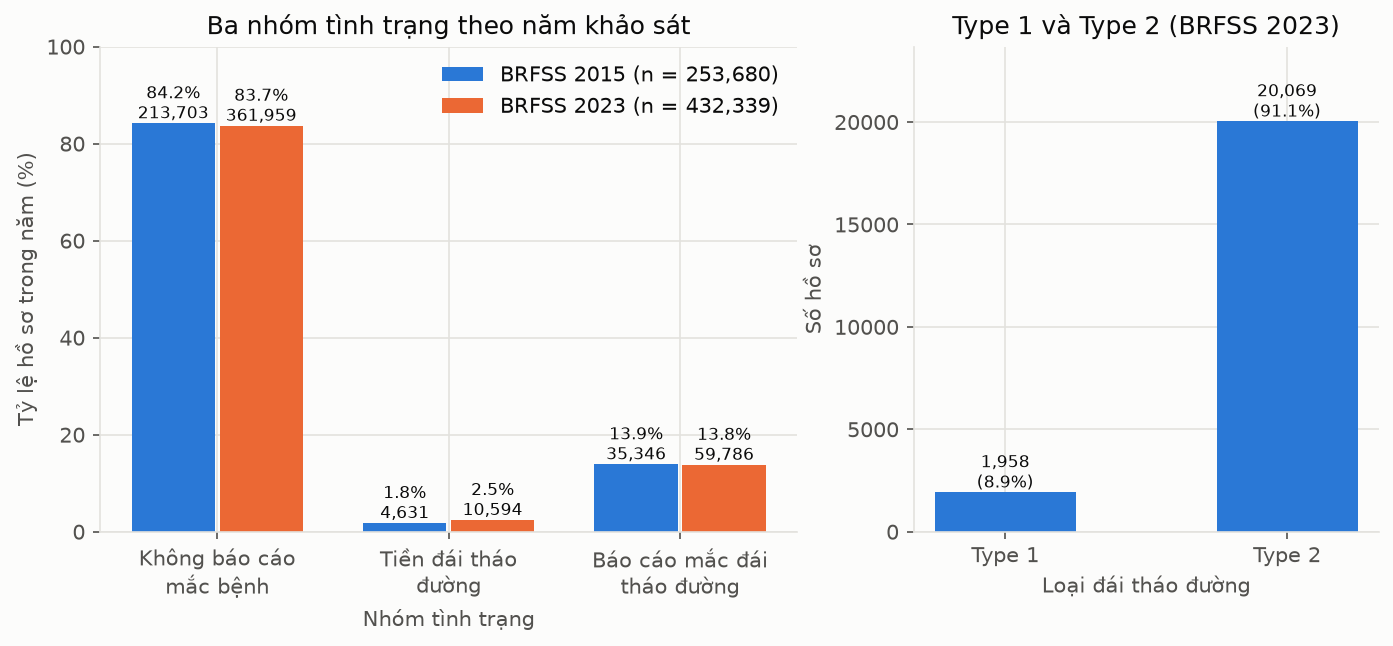
\includegraphics[width=0.78\linewidth]{../results/figures/label_distribution.png}
\caption{Phân bố nhãn của hai bài toán. Nhóm tiền đái tháo đường và nhóm Type 1 rất ít mẫu.}
\end{figure}

Cả hai bộ nhãn đều là câu trả lời tự báo cáo, không có xét nghiệm xác nhận. Nhóm tiền đái tháo đường chiếm khoảng
2\% số dòng, trong khi theo các nguồn y tế tỷ lệ thật cao hơn nhiều; phần lớn người có tiền đái tháo đường không
biết mình mắc. Vì vậy nhãn 1 ở đây là “người đã được bác sĩ thông báo có tiền đái tháo đường”, không phải
“người có tiền đái tháo đường”.

\subsection{Đặc trưng đầu vào}

Mỗi dòng có \nFeatures{} đặc trưng: huyết áp cao, cholesterol cao, đã kiểm tra cholesterol, BMI, hút thuốc, đột quỵ,
bệnh tim, hoạt động thể lực, uống nhiều rượu, có bảo hiểm y tế, không đi khám vì chi phí, tự đánh giá sức khỏe,
số ngày sức khỏe tinh thần và thể chất không tốt trong 30 ngày, khó đi lại, giới tính, nhóm tuổi, học vấn,
thu nhập. BMI (chỉ số khối cơ thể) bằng cân nặng (kg) chia bình phương chiều cao (m).

\paragraph{Ghép hai năm.}
Bộ 2015 có thêm hai cột ăn trái cây và ăn rau. Tệp năm 2023 không có câu hỏi này trong bộ 350 biến, nên hai cột bị
bỏ ở cả hai năm để mô hình nhận cùng đầu vào. Các biến năm 2023 được mã lại theo quy ước năm 2015, ví dụ
\texttt{\_BMI5} chia 100 thành BMI thật, thu nhập 11 mức của \texttt{INCOME3} gộp mức 8--11 thành mức 8;
mã 7 (không biết) và 9 (từ chối) chuyển thành giá trị thiếu. Toàn bộ bảng mã lại được lưu trong
\texttt{results/classifier.json}.

\paragraph{Tránh lộ nhãn ở bài Type 1/2.}
Các câu hỏi \texttt{DIABETE4}, \texttt{DIABAGE4} (tuổi khi được chẩn đoán) và \texttt{INSULIN1} (đang dùng insulin)
bị loại khỏi đầu vào. Câu hỏi dùng insulin gần như trả lời thẳng câu hỏi Type 1 hay Type 2, nên nếu giữ lại thì
mô hình đạt điểm cao mà không học được gì từ các đặc trưng còn lại.

\subsection{Tiền xử lý và chia tập}

\paragraph{Chia theo hồ sơ.}
Hồ sơ là toàn bộ giá trị đặc trưng của một dòng. Bộ ba nhóm có \nRowsStatus{} dòng nhưng chỉ \nProfilesStatus{} hồ sơ
khác nhau. Nếu chia ngẫu nhiên từng dòng, hai dòng giống hệt nhau có thể rơi vào tập huấn luyện và tập kiểm tra,
và mô hình được chấm trên đầu vào nó đã thấy. Chương trình gom các dòng cùng hồ sơ thành nhóm, thử 32 cách gán
nhóm vào ba tập theo tỷ lệ 70/15/15 và chọn cách có tỷ lệ từng lớp gần mục tiêu nhất; kiểm thử
\texttt{tests/test\_split.py} khẳng định không hồ sơ nào nằm ở hai tập.

\paragraph{Điền thiếu và chuẩn hóa.}
Giá trị thiếu được điền bằng trung vị của cột trên tập huấn luyện, sau đó mỗi cột được chuẩn hóa
\[ z = \frac{x - \mu}{\sigma}, \]
với $\mu$ và $\sigma$ là trung bình và độ lệch chuẩn của cột trên tập huấn luyện. Tập xác thực và kiểm tra dùng lại
đúng các thông số này; tính lại trên dữ liệu kiểm tra sẽ để lọt thông tin của tập kiểm tra vào bước học.

\begin{table}[H]
\centering
\caption{Số dòng và phân bố nhãn của từng tập (seed 0)}
\begin{tabular}{lrl}
\toprule
Bài toán / tập & Tổng & Nhãn 0 / 1 / 2 hoặc 1 / 2 \\
\midrule
\tablerows{generated/table_splits.tex}
\bottomrule
\end{tabular}
\end{table}

% ==================================================================
\section{Thiết kế hệ thống}

\subsection{Lược đồ tri thức}

\paragraph{Nút và quan hệ.}
Lược đồ quy định các loại nút, thuộc tính và quan hệ được phép. Toàn bộ lược đồ nằm trong một tệp
\texttt{backend/app/schema.py}; chương trình nạp dữ liệu, chương trình truy xuất và kiểm thử đều đọc từ tệp này,
nên đổi lược đồ ở một chỗ là đủ. Mọi nút mang thuộc tính \texttt{kb\_id = "KB\_diabet"} để phân biệt với dữ liệu
khác trong cùng cơ sở dữ liệu, và mỗi nhãn có ràng buộc duy nhất trên mã \texttt{id}.

\begin{figure}[H]
\centering
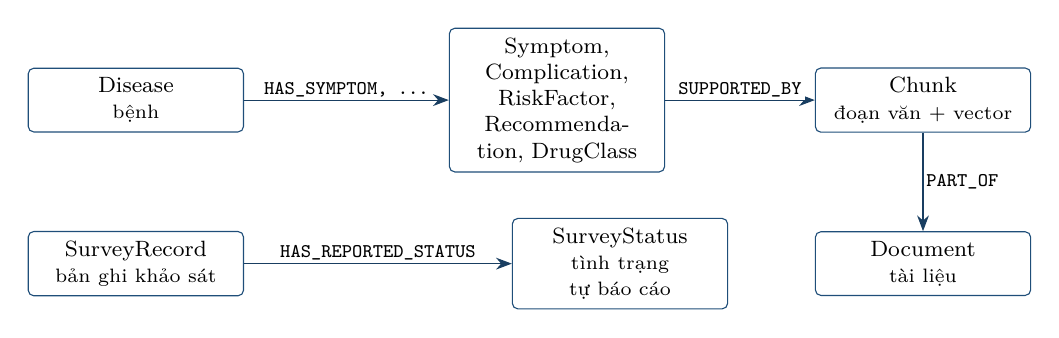
\begin{tikzpicture}[node distance=0.55cm and 1.25cm]
  \node[node] (dis) {Disease\\\scriptsize bệnh};
  \node[node, right=2.6cm of dis] (fact) {Symptom, Complication,\\RiskFactor,\\Recommendation, DrugClass};
  \node[node, right=1.9cm of fact] (chunk) {Chunk\\\scriptsize đoạn văn + vector};
  \node[node, below=1.25cm of chunk] (doc) {Document\\\scriptsize tài liệu};
  \node[node, below=1.25cm of dis] (rec) {SurveyRecord\\\scriptsize bản ghi khảo sát};
  \node[node, right=3.4cm of rec] (st) {SurveyStatus\\\scriptsize tình trạng tự báo cáo};
  \draw[arr] (dis) -- node[lab, above] {HAS\_SYMPTOM, ...} (fact);
  \draw[arr] (fact) -- node[lab, above] {SUPPORTED\_BY} (chunk);
  \draw[arr] (chunk) -- node[lab, right] {PART\_OF} (doc);
  \draw[arr] (rec) -- node[lab, above] {HAS\_REPORTED\_STATUS} (st);
\end{tikzpicture}
\caption{Lược đồ đồ thị \texttt{KB\_diabet}. Quan hệ \texttt{SUPPORTED\_BY} mang thuộc tính \texttt{quote}: câu trích nguyên văn.}
\end{figure}

\begin{table}[H]
\centering
\begin{minipage}[t]{0.42\linewidth}\centering
\captionof{table}{Số nút theo nhãn}
\begin{tabular}{lr}
\toprule
Nhãn & Số nút \\
\midrule
\tablerows{generated/table_nodes.tex}
\bottomrule
\end{tabular}
\end{minipage}\hfill
\begin{minipage}[t]{0.52\linewidth}\centering
\captionof{table}{Số quan hệ theo loại}
\begin{tabular}{lr}
\toprule
Quan hệ & Số lượng \\
\midrule
\tablerows{generated/table_rels.tex}
\bottomrule
\end{tabular}
\end{minipage}
\end{table}

\subsection{Trích dữ kiện y tế có kiểm chứng}

Mỗi đoạn văn được gửi cho mô hình ngôn ngữ \texttt{\llmModel} kèm yêu cầu liệt kê các dữ kiện đoạn nêu rõ, ở dạng
JSON: loại dữ kiện, bệnh liên quan, tên ngắn tiếng Việt, điều kiện áp dụng nếu có, và một câu trích nguyên văn từ
đoạn. Mô hình ngôn ngữ có thể bịa câu trích, nên chương trình không tin kết quả này mà kiểm lại bằng code: câu trích
phải là một chuỗi con của đoạn văn sau khi chuẩn hóa khoảng trắng và chữ hoa. Dữ kiện không qua bước kiểm bị loại và
ghi vào \texttt{results/facts\_rejected.jsonl}.

\begin{softbox}
Trên toàn kho, mô hình đề xuất \nProposed{} dữ kiện. Chương trình giữ \nAccepted{}, loại \nRejQuote{} dữ kiện có câu
trích không nằm trong đoạn và \nRejOther{} dữ kiện sai loại hoặc sai mã bệnh. Bước này tốn \extractTokens{} token.
\end{softbox}

Dữ kiện trùng tên được gộp thành một nút, kể cả khi đến từ hai nguồn khác nhau; một bảng đồng nghĩa nhỏ
(\texttt{pipeline/synonyms.yaml}) gộp các cách gọi khác nhau như “khát nước nhiều” và “khát nhiều”. Khi một
khuyến nghị được nhiều nguồn cùng nêu, nút khuyến nghị có nhiều quan hệ \texttt{SUPPORTED\_BY}, mỗi quan hệ tới
một đoạn văn. Ví dụ nút “giảm cân nếu thừa cân và duy trì cân nặng đó” được cả NIDDK và NDSS hỗ trợ.

\paragraph{Giới hạn.}
Tên ngắn do mô hình đặt không thống nhất giữa các lần gọi, nên việc gộp còn yếu: trong \nFacts{} dữ kiện chỉ
\nBilingualFacts{} dữ kiện được nguồn của cả hai ngôn ngữ cùng hỗ trợ. Một số dữ kiện bị gán sai loại, ví dụ cụm
“không cần liệu pháp insulin” bị xếp vào triệu chứng của đái tháo đường típ 2. Bước kiểm câu trích đảm bảo dữ kiện
có trong nguồn, nhưng không kiểm được dữ kiện có được phân loại đúng hay không.

\subsection{Dữ liệu khảo sát trên đồ thị}

Bộ khảo sát được nạp vào tệp SQLite \texttt{data/survey.db} gồm bảng \texttt{survey\_records} (mã dòng, năm, nhãn,
bài toán và các đặc trưng dạng JSON) và bảng \texttt{status\_definitions} (mô tả nhãn). Chương trình lấy tối đa 100
dòng đầu cho mỗi cặp năm và nhãn, tạo nút \texttt{SurveyRecord} và nối tới nút \texttt{SurveyStatus} tương ứng.
Lệnh \texttt{MERGE} của Neo4j tìm nút theo khóa và chỉ tạo khi chưa có, nên chạy lại không sinh nút trùng;
kiểm thử \texttt{tests/test\_ingest\_idempotent.py} chạy nạp hai lần và so số nút.

Mẫu 600 dòng trên đồ thị chỉ minh họa luồng nạp dữ liệu quan hệ. Hai bộ phân loại được huấn luyện trên toàn bộ dữ liệu.

\subsection{Kiến trúc xử lý}

\begin{figure}[H]
\centering
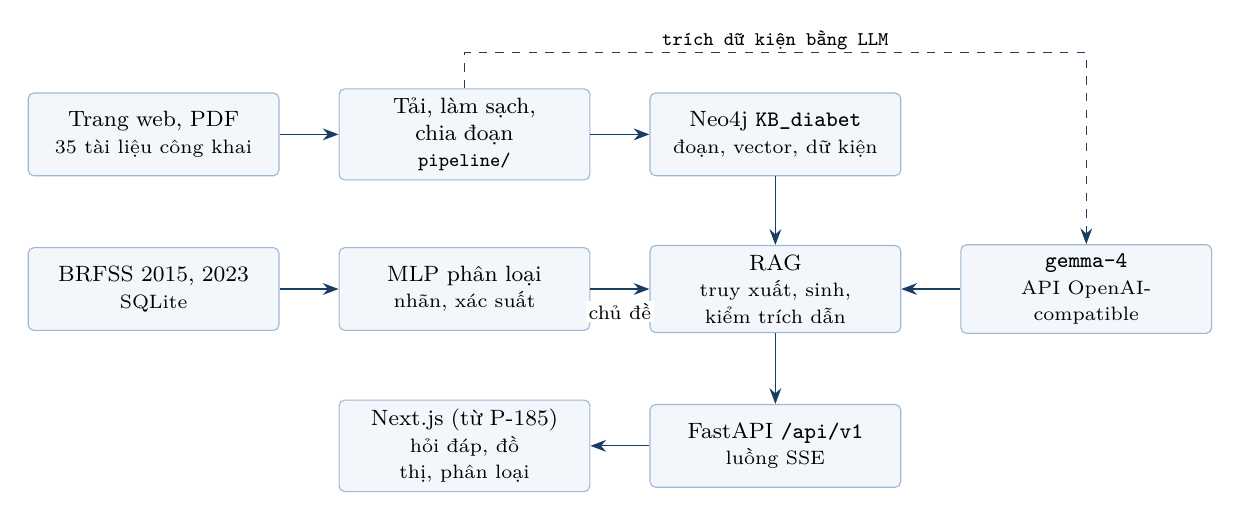
\begin{tikzpicture}[node distance=0.9cm and 0.75cm, box/.append style={text width=2.95cm}]
  \node[box] (src) {Trang web, PDF\\\scriptsize \nDocs{} tài liệu công khai};
  \node[box, right=of src] (clean) {Tải, làm sạch, chia đoạn\\\scriptsize \texttt{pipeline/}};
  \node[box, right=of clean] (neo) {Neo4j \texttt{KB\_diabet}\\\scriptsize đoạn, vector, dữ kiện};
  \node[box, below=of src] (csv) {BRFSS 2015, 2023\\\scriptsize SQLite};
  \node[box, right=of csv] (mlp) {MLP phân loại\\\scriptsize nhãn, xác suất};
  \node[box, right=of mlp] (rag) {RAG\\\scriptsize truy xuất, sinh, kiểm trích dẫn};
  \node[box, right=of rag] (llm) {\texttt{\llmModel}\\\scriptsize API OpenAI-compatible};
  \node[box, below=of rag] (api) {FastAPI \texttt{/api/v1}\\\scriptsize luồng SSE};
  \node[box, left=of api] (web) {Next.js (từ P-185)\\\scriptsize hỏi đáp, đồ thị, phân loại};
  \draw[arr] (src) -- (clean);
  \draw[arr] (clean) -- (neo);
  \draw[arr] (csv) -- (mlp);
  \draw[arr] (neo) -- (rag);
  \draw[arr] (mlp) -- (rag) node[lab, midway, below=4pt, font=\scriptsize] {chủ đề};
  \draw[arr] (llm) -- (rag);
  \draw[arr] (rag) -- (api);
  \draw[arr] (api) -- (web);
  \draw[arr, dashed] (clean.north) -- ++(0,0.45) -| node[lab, pos=0.25, above] {trích dữ kiện bằng LLM} (llm.north);
\end{tikzpicture}
\caption{Kiến trúc thu thập, phân loại và hỏi đáp.}
\end{figure}

\paragraph{Kế thừa từ P-185.}
Kiến trúc và giao diện được dựng lại từ P-185, một trợ lý tra cứu pháp luật thuế cùng dạng bài toán (câu trả lời
phải có căn cứ trích dẫn). Bài làm giữ lại các phần dùng chung được: hợp đồng sự kiện SSE giữa máy chủ và trình
duyệt, bộ phân tích luồng sự kiện phía trình duyệt, khung trò chuyện, bảng nguồn, hệ màu và phông chữ. Các phần
gắn với nghiệp vụ thuế (tờ khai, máy tính thuế, phân quyền kế toán, hiệu lực văn bản) và các phần không cần cho
bài (PostgreSQL, đăng nhập, LangGraph) được bỏ. Phía máy chủ được viết lại gọn; mã giao diện còn khoảng 3.400 dòng
so với khoảng 44.000 dòng của bản gốc.

\paragraph{Luồng sự kiện SSE.}
SSE (Server-Sent Events) là cách máy chủ gửi dần từng sự kiện qua một kết nối HTTP. Một lượt hỏi phát lần lượt
\texttt{stream.started}, \texttt{sources.snapshot} (các đoạn đã tìm được), \texttt{answer.started}, các sự kiện
\texttt{answer.text.delta} và \texttt{answer.citation}, \texttt{answer.final} (câu trả lời đầy đủ) và
\texttt{stream.completed}. Kiểm thử phía giao diện so danh sách tên sự kiện với \texttt{schema.py} để hai phía
không lệch nhau.

% ==================================================================
\section{Hệ thống hỏi đáp RAG}

\subsection{Truy xuất nội dung}

\paragraph{Biểu diễn văn bản.}
Biểu diễn số (embedding) chuyển một đoạn văn thành vector, tức một dãy số có thứ tự. Bài làm dùng mô hình
\texttt{BAAI/bge-m3}, tạo vector \embedDim{} số cho mỗi đoạn, được huấn luyện để câu hỏi và đoạn văn cùng nghĩa có
vector gần nhau kể cả khi khác ngôn ngữ. Vector được lưu ngay trên thuộc tính \texttt{embedding} của nút
\texttt{Chunk} và đánh chỉ mục vector của Neo4j, nên không cần một cơ sở dữ liệu vector riêng. Độ gần được đo
bằng cosine:
\[ \cos(u, v) = \frac{\sum_i u_i v_i}{\sqrt{\sum_i u_i^2}\,\sqrt{\sum_i v_i^2}}. \]
Các vector được chuẩn hóa về độ dài 1, nên cosine bằng tích vô hướng.

\paragraph{Ba nhánh truy xuất.}
Chương trình có ba cách tìm đoạn văn:
\begin{itemize}
  \item \textbf{BM25}: chấm điểm theo số từ chung giữa câu hỏi và đoạn, có trọng số cho từ hiếm.
  \item \textbf{Vector}: lấy 20 đoạn có cosine cao nhất qua chỉ mục vector của Neo4j.
  \item \textbf{Đồ thị}: từ các đoạn tốt nhất, đi theo \texttt{SUPPORTED\_BY} tới dữ kiện rồi đi tiếp tới các đoạn
        khác hỗ trợ cùng dữ kiện; nếu biết chủ đề, lấy thêm các đoạn hỗ trợ dữ kiện của bệnh tương ứng.
\end{itemize}
Khi dùng nhiều nhánh, danh sách được gộp bằng RRF (Reciprocal Rank Fusion): đoạn ở hạng $r$ của một nhánh nhận
điểm $1/(k + r)$ với $k = \rrfK$, và điểm của đoạn là tổng điểm qua các nhánh.

\paragraph{Cấu hình được chọn.}
Mục~\ref{sec:retrieval} cho thấy xếp hạng chỉ bằng vector cho kết quả tốt nhất, và đưa đồ thị vào làm một nhánh xếp
hạng ngang hàng làm kết quả kém đi. Vì vậy cấu hình chạy thật xếp hạng bằng vector, lấy 5 đoạn đầu, rồi dùng đồ thị
theo hai cách không làm xáo trộn thứ hạng: gắn các dữ kiện (kèm điều kiện áp dụng) của mỗi đoạn vào ngữ cảnh, và nối
thêm tối đa \expandN{} đoạn liên kết qua dữ kiện chung vào sau 5 đoạn đầu.

\subsection{Sinh câu trả lời và kiểm trích dẫn}

\paragraph{Lời nhắc.}
Các đoạn được đánh nhãn S1, S2, \dots{} và gửi cho mô hình cùng câu hỏi. Lời nhắc yêu cầu chỉ dùng thông tin trong
nguồn, đặt dấu \texttt{[[cite:Sn]]} sau mỗi ý, giữ nguyên điều kiện áp dụng, không thêm liều thuốc hay con số không
có trong nguồn, và viết đúng một dòng \texttt{KHONG\_DU\_BANG\_CHUNG} khi nguồn không trả lời được câu hỏi.

\paragraph{Cổng trích dẫn.}
Trước khi hiển thị, chương trình chuẩn hóa mọi cách viết trích dẫn của mô hình (\texttt{[[S5]]}, \texttt{[S1]},
\texttt{[[1, 3]]}) về một dạng, bỏ các trích dẫn trỏ tới nguồn không được cung cấp, và chuyển câu trả lời không còn
trích dẫn hợp lệ nào thành trạng thái \texttt{insufficient\_evidence}. Câu hỏi có cosine cao nhất dưới \oosMin{}
được coi là ngoài phạm vi và bị từ chối mà không gọi mô hình. Vì cổng chạy trên toàn bộ câu trả lời, máy chủ đợi mô
hình viết xong rồi mới phát các đoạn chữ; người dùng không bao giờ thấy một ý chưa qua kiểm tra.

\begin{table}[H]
\centering
\caption{Ba trạng thái câu trả lời}
\begin{tabularx}{\linewidth}{L{4.3cm}Y}
\toprule
Trạng thái & Ý nghĩa \\
\midrule
\texttt{answered} & Có ít nhất một trích dẫn hợp lệ; giao diện hiện phần trả lời và phần căn cứ. \\
\texttt{insufficient\_evidence} & Câu hỏi trong lĩnh vực nhưng nguồn tìm được không trả lời được. \\
\texttt{out\_of\_scope} & Câu hỏi không gần nội dung nào của kho; không gọi mô hình ngôn ngữ. \\
\bottomrule
\end{tabularx}
\end{table}

\subsection{Phương pháp đánh giá}
\label{sec:method}

\paragraph{Bộ câu hỏi.}
Bộ đánh giá gồm \nQuestions{} câu: \nInScope{} câu trong phạm vi (khái niệm, triệu chứng, nguy cơ, chẩn đoán, ăn uống,
vận động, thuốc, biến chứng, tổng hợp; trong đó \nQEn{} câu tiếng Anh) và \nOos{} câu ngoài phạm vi, gồm hai câu
gần lĩnh vực (ung thư tuyến tụy, thuốc cảm cúm).

\paragraph{Tham chiếu theo nội dung.}
Với mỗi câu, chương trình gộp 20 đoạn đầu của mọi nhánh truy xuất (trung bình \poolMean{} đoạn), và mô hình ngôn ngữ
chấm từng đoạn có chứa câu trả lời trực tiếp hay không. Bộ chấm phải trích nguyên văn câu trả lời trong đoạn, và
chương trình kiểm câu trích có thật trong đoạn. Kết quả là \nGoldPairs{} cặp câu hỏi và đoạn liên quan, từ \goldMin{}
đến \goldMax{} đoạn mỗi câu, bằng cả hai ngôn ngữ. Đọc lại \relAgree{} nhãn dương ngẫu nhiên thấy khớp với đánh giá
của người đọc; trước khi thêm bước kiểm câu trích, tỷ lệ này chỉ khoảng \relAgreeLenient{}.

\paragraph{Chỉ số truy xuất.}
Với $R$ là tập đoạn liên quan và $T_k$ là $k$ đoạn đầu chương trình trả về:
\begin{align*}
\text{Hit@}k &= \mathbb{1}\!\left[\,|R \cap T_k| > 0\,\right], &
\text{Precision@}k &= \frac{|R \cap T_k|}{k}, \\
\text{Recall@}k &= \frac{|R \cap T_k|}{\min(|R|, k)}, &
\text{MRR} &= \frac{1}{\text{hạng của đoạn liên quan đầu tiên}}.
\end{align*}
Recall@$k$ chia cho $\min(|R|, k)$ thay vì $|R|$: một câu có 20 đoạn liên quan thì 5 kết quả đầu không thể chứa đủ
20, và chia cho 20 sẽ phạt hệ thống vì điều nó không làm được. Ví dụ với $R = \{a, b\}$ và kết quả $\{a, c, d\}$:
Hit@3 $= 1$, Precision@3 $= 1/3$, Recall@3 $= 1/2$, MRR $= 1$ (kiểm thử \texttt{tests/test\_metrics.py}).

\paragraph{Chất lượng câu trả lời.}
Mô hình chấm tách câu trả lời thành các phát biểu đơn và xét từng phát biểu với \emph{toàn văn} các đoạn nó trích:
được hỗ trợ, hỗ trợ một phần, hoặc không được hỗ trợ. Đọc lại \claimAgree{} phát biểu ngẫu nhiên và tra nguồn thấy
khớp với bộ chấm. Bộ chấm chỉ xét phát biểu có căn cứ hay không, chưa xét phát biểu có trả lời đúng trọng tâm câu
hỏi hay không.

% ==================================================================
\section{Thực nghiệm phân loại}

\subsection{Môi trường và cấu hình}

Thực nghiệm chạy trên máy Apple M2, Python 3.11, PyTorch, CPU. Hai mốc so sánh là mô hình luôn đoán lớp đông nhất
và hồi quy logistic có trọng số lớp cân bằng. MLP có hai lớp ẩn 64 và 32 đơn vị:
\[ h = \mathrm{ReLU}(Wx + b), \qquad \mathrm{ReLU}(a) = \max(0, a), \]
dropout 0,15, thuật toán Adam với tốc độ học 0,001, lô 512 dòng, tối đa 40 lượt học, dừng khi macro-F1 trên tập xác
thực không tăng sau 7 lượt và khôi phục trọng số tốt nhất. Hàm mất mát là cross entropy có trọng số
$\ell_i = -w_{y_i}\log p_{i, y_i}$, trọng số lớp tỷ lệ nghịch với tần suất lớp trong tập huấn luyện. Toàn bộ năm seed
của hai bài chạy trong \trainSeconds{} giây.

\subsection{Chỉ số}

Accuracy là tỷ lệ dự đoán đúng trên toàn bộ mẫu. Với một lớp, precision $= TP/(TP+FP)$ là tỷ lệ đúng trong các mẫu
được dự đoán vào lớp đó, recall $= TP/(TP+FN)$ là tỷ lệ mẫu thật của lớp được tìm ra, và F1 là trung bình điều hòa
của hai chỉ số này. Macro-F1 lấy trung bình F1 các lớp với trọng số ngang nhau, nên lớp ít mẫu có ảnh hưởng ngang lớp
đông mẫu. Khi một lớp chiếm hơn 80\% mẫu, accuracy có thể cao dù mô hình bỏ sót hoàn toàn các lớp còn lại, nên bài
làm chọn mô hình và so sánh bằng macro-F1.

\subsection{So sánh mô hình}

Mỗi mô hình được huấn luyện với 5 seed (0 đến 4). Mỗi seed vẽ lại cách chia tập, nên độ lệch chuẩn bao gồm cả dao
động do chia tập.

\begin{table}[H]
\centering
\caption{Kết quả trên tập kiểm tra, trung bình $\pm$ độ lệch chuẩn qua 5 seed}
\begin{tabular}{lcc}
\toprule
Mô hình & Accuracy & Macro-F1 \\
\midrule
\multicolumn{3}{l}{\itshape Ba nhóm tình trạng} \\
\tablerows{generated/table_clf_status.tex}
\midrule
\multicolumn{3}{l}{\itshape Type 1 / Type 2} \\
\tablerows{generated/table_clf_type.tex}
\bottomrule
\end{tabular}
\end{table}

Mô hình luôn đoán lớp đông nhất có accuracy cao nhất ở cả hai bài nhưng macro-F1 thấp nhất. Trọng số lớp đổi một
phần accuracy lấy khả năng tìm ra các lớp ít mẫu. Ở bài ba nhóm, MLP và hồi quy logistic có macro-F1 chênh nhau ít hơn
một độ lệch chuẩn, nên thí nghiệm không cho thấy MLP tốt hơn. Ở bài Type 1/2, MLP cao hơn logistic khoảng hai độ
lệch chuẩn.

\subsection{Kết quả ba nhóm khảo sát}

\begin{figure}[H]
\centering
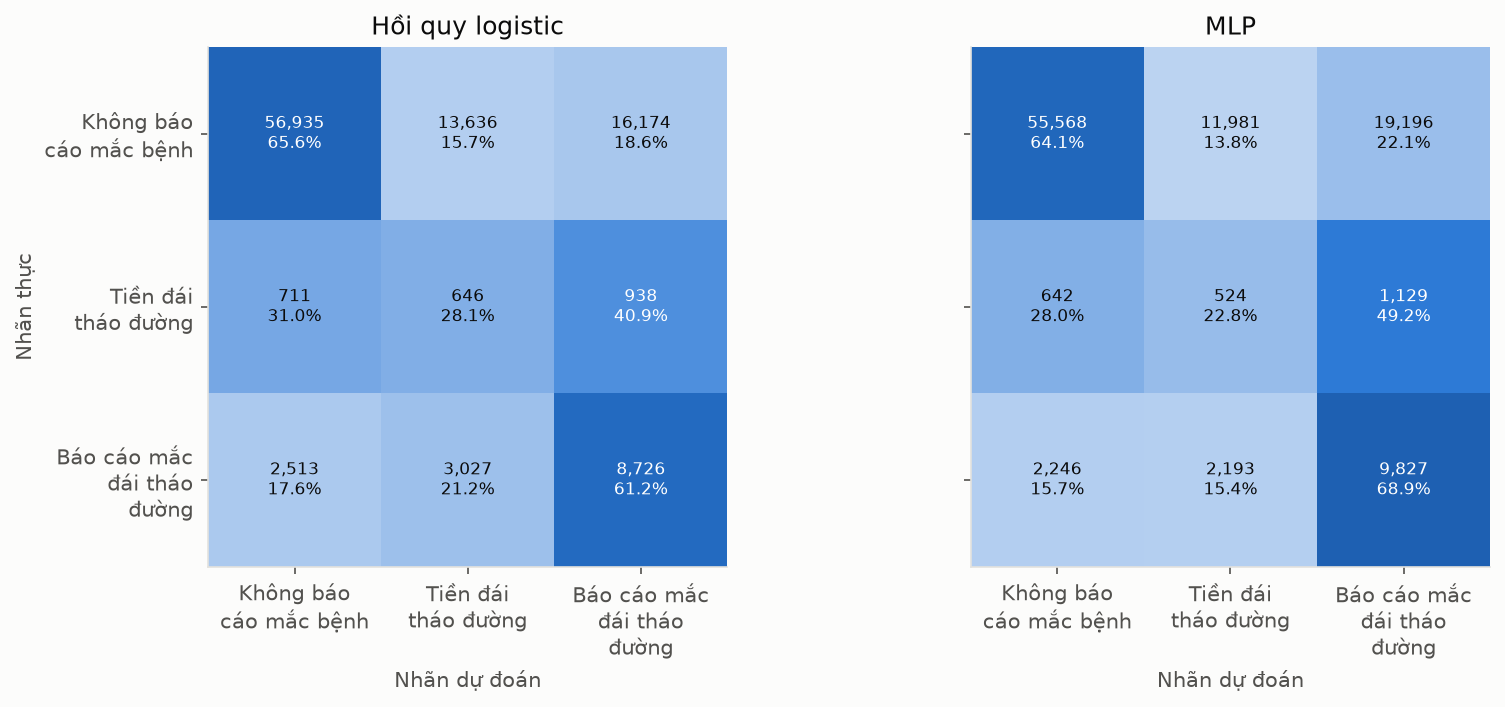
\includegraphics[width=0.62\linewidth]{../results/figures/confusion_status3.png}
\caption{Ma trận nhầm lẫn trên tập kiểm tra ba nhóm (seed 0): hồi quy logistic (trái) và MLP (phải). Hàng là nhãn thật, cột là nhãn dự đoán.}
\end{figure}

\begin{table}[H]
\centering
\caption{Chỉ số từng lớp của MLP (seed 0), bài ba nhóm}
\begin{tabular}{lrrrr}
\toprule
Lớp & Precision & Recall & F1 & Số mẫu \\
\midrule
\tablerows{generated/table_class_status.tex}
\bottomrule
\end{tabular}
\end{table}

Lớp tiền đái tháo đường gần như không học được: mô hình nhận đúng \preTP{} trên \preSupport{} mẫu, và chỉ
\prePrecision{} số dự đoán vào lớp này là đúng. Đầu vào không có xét nghiệm đường huyết hay HbA1c, và nhãn lớp này
phụ thuộc vào việc người trả lời đã từng được bác sĩ thông báo hay chưa, điều mà các đặc trưng hiện có không mô tả.

\begin{figure}[H]
\centering
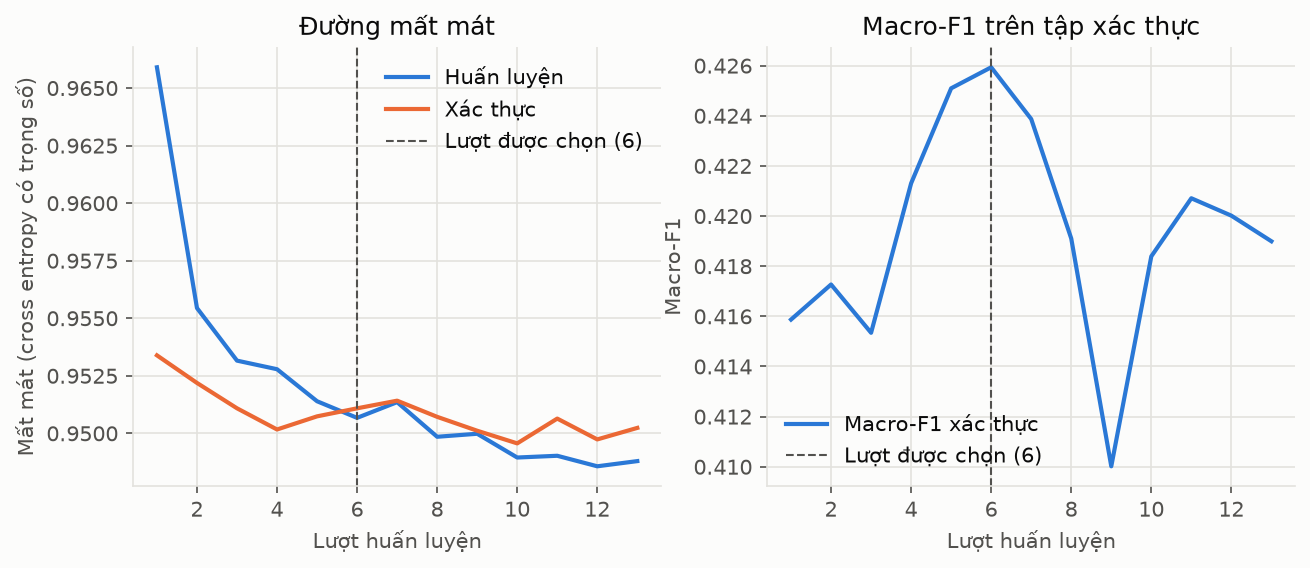
\includegraphics[width=0.49\linewidth]{../results/figures/learning_curves_status3.png}\hfill
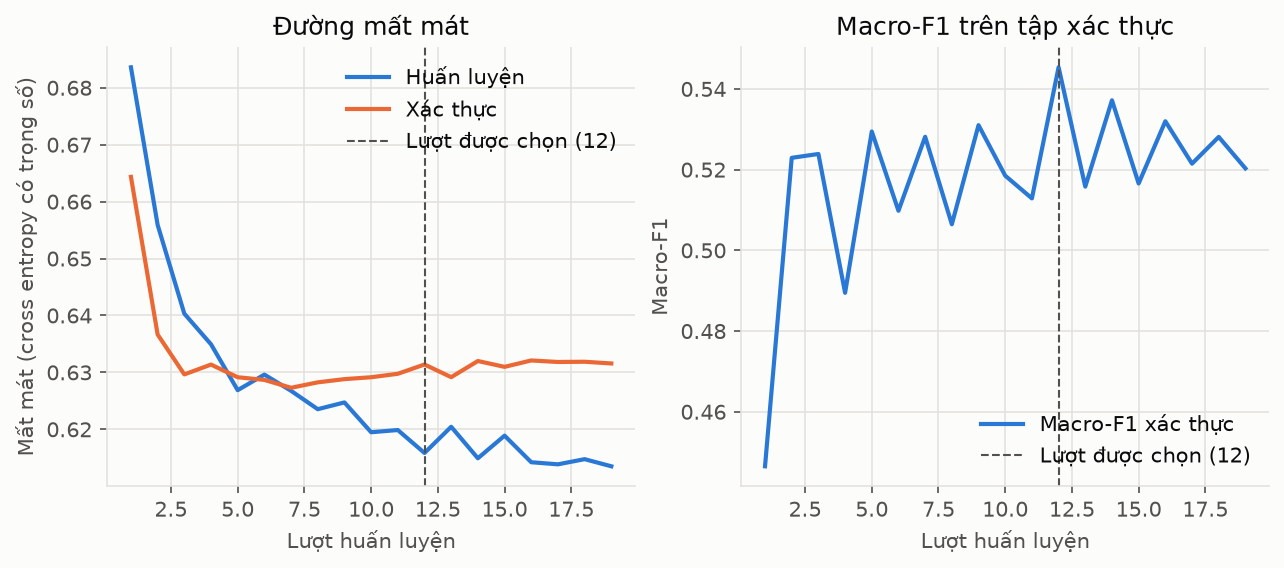
\includegraphics[width=0.49\linewidth]{../results/figures/learning_curves_diabtype.png}
\caption{Sai số học, sai số xác thực và macro-F1 xác thực của MLP (seed 0): ba nhóm (trái), Type 1/2 (phải).}
\end{figure}

Ở bài ba nhóm, macro-F1 xác thực cao nhất ở lượt \bestEpochStatus{} và chương trình dừng ở lượt \epochsStatus{};
ở bài Type 1/2 là lượt \bestEpochType{} và \epochsType{}. Sai số học tiếp tục giảm trong khi sai số xác thực đi
ngang, nên học thêm không cải thiện trên dữ liệu chưa thấy.

\subsection{Kết quả Type 1 / Type 2}

\begin{figure}[H]
\centering
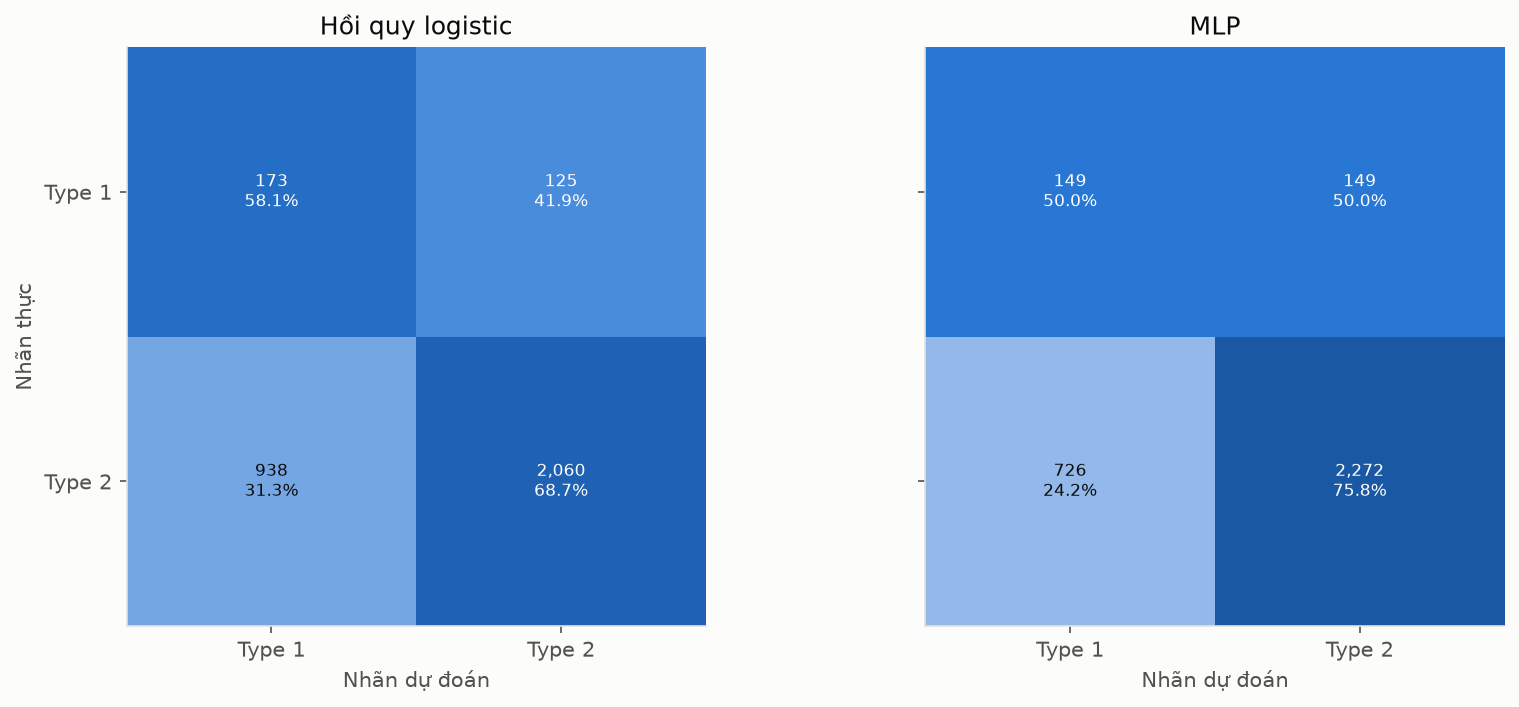
\includegraphics[width=0.5\linewidth]{../results/figures/confusion_diabtype.png}
\caption{Ma trận nhầm lẫn bài Type 1/2 (seed 0): hồi quy logistic (trái) và MLP (phải).}
\end{figure}

\begin{table}[H]
\centering
\caption{Chỉ số từng lớp của MLP (seed 0), bài Type 1/2}
\begin{tabular}{lrrrr}
\toprule
Lớp & Precision & Recall & F1 & Số mẫu \\
\midrule
\tablerows{generated/table_class_type.tex}
\bottomrule
\end{tabular}
\end{table}

Mô hình nhận đúng \typeOneTP{} trên \typeOneSupport{} mẫu Type 1, nhưng trong \typeOnePred{} lần dự đoán Type 1 chỉ
\typeOnePrecision{} là đúng. Tỷ lệ báo động sai này cho thấy nhãn dự đoán không đủ tin cậy để kết luận loại bệnh của
một người; hệ thống chỉ dùng nó để gợi ý chủ đề đọc.

\subsection{Hiệu chỉnh xác suất}

Xác suất đầu ra của mô hình được hiển thị trên giao diện, nên cần biết nó có phản ánh đúng tần suất thật hay không.
ECE (expected calibration error) chia dự đoán thành 15 khoảng theo độ tự tin và lấy trung bình có trọng số của độ
chênh giữa độ tự tin và tỷ lệ đúng trong từng khoảng. Temperature scaling chia điểm đầu ra cho một hằng số $T$
chọn trên tập xác thực.

\begin{table}[H]
\centering
\caption{ECE trên tập kiểm tra (MLP, seed 0)}
\begin{tabular}{lcccc}
\toprule
Bài toán & $T$ & Trước & Sau temperature scaling & Sau khi bỏ trọng số lớp \\
\midrule
Ba nhóm & \tempStatus & \eceStatusBefore & \eceStatusAfter & \eceStatusPrior \\
Type 1/2 & \tempType & \eceTypeBefore & \eceTypeAfter & \eceTypePrior \\
\bottomrule
\end{tabular}
\end{table}

Temperature scaling giảm ECE nhưng không xóa được độ lệch do trọng số lớp gây ra: trọng số lớp cố ý đẩy xác suất về
phía các lớp hiếm. Cột cuối là phép đo chẩn đoán, khi bỏ ảnh hưởng của trọng số lớp khỏi xác suất; ECE giảm rõ.
Giao diện hiện dùng xác suất sau temperature scaling, và kèm lời nhắc rằng đây không phải kết quả chẩn đoán.

% ==================================================================
\section{Kết quả hỏi đáp}

\subsection{So sánh các cách truy xuất}
\label{sec:retrieval}

\begin{table}[H]
\centering
\caption{Truy xuất trên \nInScope{} câu trong phạm vi, xếp hạng 10 đoạn, không mở rộng}
\begin{tabular}{lccccc}
\toprule
Cấu hình & Hit@3 & Hit@5 & Precision@5 & Recall@5 & MRR@10 \\
\midrule
\tablerows{generated/table_retrieval.tex}
\bottomrule
\end{tabular}
\end{table}

\begin{figure}[H]
\centering
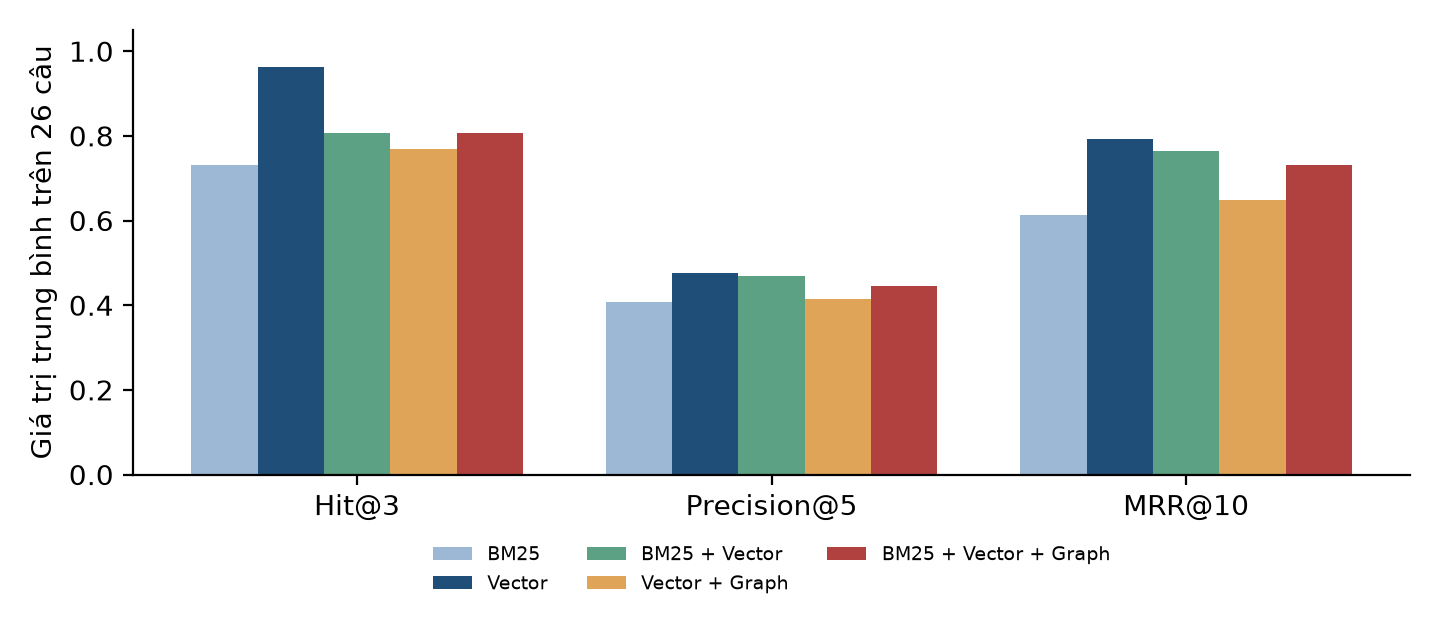
\includegraphics[width=0.85\linewidth]{generated/retrieval_ablation.png}
\caption{Ba chỉ số truy xuất theo cấu hình.}
\end{figure}

Vector đứng đầu ở mọi chỉ số; năm đoạn đầu chứa ít nhất một đoạn liên quan ở tất cả \nInScope{} câu. Thêm BM25 làm
kết quả kém đi. BM25 tách tiếng Việt theo âm tiết, và các âm tiết như “đái”, “tháo”, “đường” xuất hiện ở hầu hết
mọi đoạn nên đóng góp nhiều nhiễu. Thêm đồ thị vào RRF như một nhánh ngang hàng cũng làm kết quả kém đi: nhánh đồ
thị trả về các đoạn hỗ trợ cùng dữ kiện, nhưng “cùng dữ kiện” không có nghĩa là “trả lời cùng câu hỏi”, và các
đoạn này đẩy đoạn tốt của vector xuống dưới.

Cần lưu ý một điểm về cách đo. Tập tham chiếu được gộp từ 20 đoạn đầu của mọi nhánh, nên không thiên về một nhánh
nào ở bước chọn ứng viên; nhưng bộ chấm và bộ biểu diễn đều là mô hình học sâu, và đoạn được vector xếp cao có thể
cũng dễ được bộ chấm coi là liên quan.

\subsection{Đóng góp của đồ thị}

Đồ thị được dùng theo cách khác: nối thêm tối đa \expandN{} đoạn sau 5 đoạn đầu của vector. Trên \nInScope{} câu, đồ
thị thêm \gxAdded{} đoạn; \gxRelevant{} trong số đó liên quan đến câu hỏi, \gxOther{} là đoạn ở ngôn ngữ còn lại,
và \gxNew{} đoạn liên quan nằm ngoài 10 đoạn đầu của vector, tức là vector không tìm được.

\begin{table}[H]
\centering
\caption{Câu trả lời có và không có mở rộng bằng đồ thị}
\begin{tabular}{lcc}
\toprule
Chỉ số & Không mở rộng & Mở rộng \expandN{} đoạn \\
\midrule
Câu trong phạm vi được trả lời & \answeredZero & \answeredTwo \\
Số phát biểu được chấm & \claimsZero & \claimsTwo \\
Phát biểu được nguồn hỗ trợ & \supportedZero & \supportedTwo \\
Phát biểu không được hỗ trợ & \unsupportedZero & \unsupportedTwo \\
Từ chối nhầm câu trong phạm vi & \falseRefusalZero & \falseRefusalTwo \\
\bottomrule
\end{tabular}
\end{table}

Hai cấu hình chênh nhau một câu hỏi trên một lần chạy, nên thí nghiệm không cho thấy đồ thị cải thiện câu trả lời
một cách đo được. Kết quả cho thấy việc mở rộng không làm câu trả lời kém đi và có đưa thêm bằng chứng từ ngôn ngữ
còn lại, nên cấu hình chạy thật giữ lại bước mở rộng.

\subsection{Chất lượng câu trả lời}

Với cấu hình chạy thật, hệ thống trả lời \answeredTwo{} câu trong phạm vi, từ chối đúng \refusalOos{} câu ngoài phạm
vi, và \supportedTwo{} phát biểu được nguồn trích dẫn hỗ trợ. Thời gian một câu có trung vị \latencyP{} giây, lâu nhất
\latencyMax{} giây, phần lớn là thời gian mô hình ngôn ngữ viết câu trả lời.

\paragraph{Các lỗi đã tìm ra trong quá trình đo.}
Số liệu trên là kết quả sau ba vòng đo và sửa; hai vòng đầu là lỗi của hệ thống đo và của cổng trích dẫn, không phải
của mô hình.
\begin{enumerate}
  \item Lần đo đầu cho \vZeroUnsupported{} phát biểu không được hỗ trợ. Nguyên nhân là bộ chấm chỉ nhận 600 ký tự đầu
        của mỗi nguồn, trong khi một đoạn dài hơn nhiều. Sau khi cho bộ chấm đọc toàn văn, tỷ lệ này còn \vOneUnsupported{}.
  \item Tỷ lệ từ chối nhầm câu trong phạm vi khi đó là \vOneFalseRefusal{}. Đọc đầu ra thô cho thấy mô hình viết trích
        dẫn dạng \texttt{[[S5]]}, \texttt{[[1, 3, 5]]} hay \texttt{[[S2, S4]]}, và cổng trích dẫn xóa hết vì không khớp
        dạng \texttt{[[cite:S5]]}. Sau khi cổng chuẩn hóa các cách viết này, tỷ lệ từ chối nhầm còn \falseRefusalTwo{}.
\end{enumerate}

\begin{figure}[H]
\centering
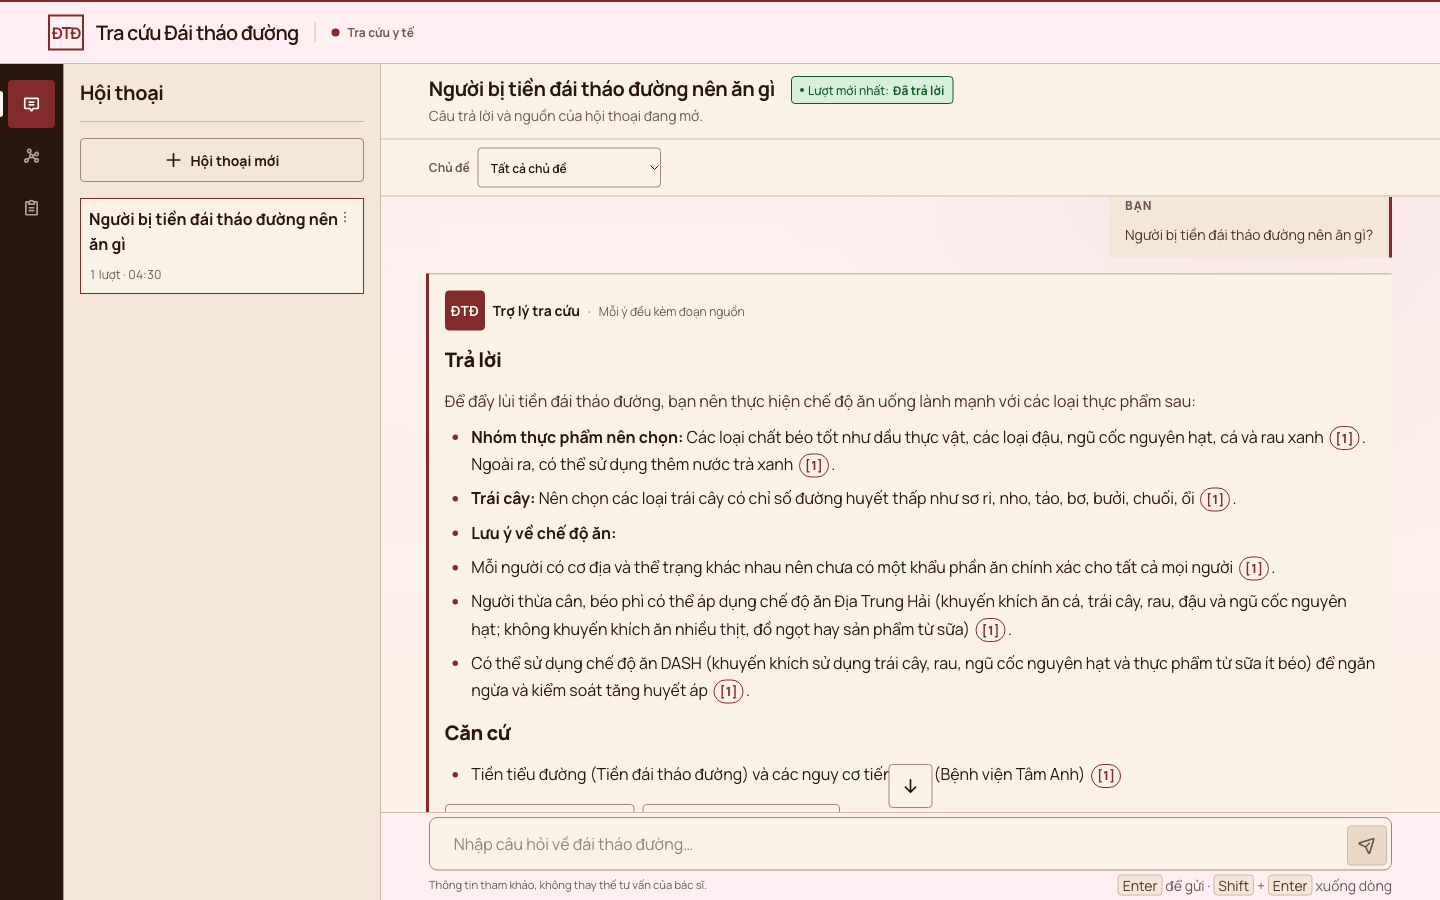
\includegraphics[width=0.95\linewidth]{../results/screens/u7b/chat-diet.png}
\caption{Giao diện hỏi đáp chạy với dữ liệu thật: câu trả lời có trích dẫn đánh số, phần căn cứ ghi tài liệu và đơn vị xuất bản.}
\end{figure}

% ==================================================================
\section{Tích hợp và thảo luận}

\subsection{Phân loại và chọn chủ đề}

Nhãn dự đoán được chuyển thành chủ đề qua một bảng duy nhất trong \texttt{schema.py}: nhãn 0 thành chủ đề phòng ngừa,
nhãn 1 thành tiền đái tháo đường, nhãn 2 thành đái tháo đường nói chung, Type 1 và Type 2 thành chủ đề tương ứng.
Kiểm thử khẳng định mọi nhãn mà bộ phân loại có thể trả ra đều có trong bảng. Trên trang phân loại, nút
“Tra cứu theo chủ đề này” mở trang hỏi đáp với chủ đề đã chọn; chủ đề được truyền vào bước mở rộng đồ thị để lấy
thêm các đoạn hỗ trợ dữ kiện của bệnh tương ứng.

Với hồ sơ minh họa BMI 40, nhóm tuổi 9 (60--64 tuổi), huyết áp cao và cholesterol cao, mô hình ba nhóm dự đoán nhãn 2
(báo cáo mắc đái tháo đường) và hệ thống mở chủ đề đái tháo đường nói chung. Nhãn này không xác định Type 1 hay Type 2;
bài Type 1/2 dùng mô hình và đầu vào riêng, chỉ có nghĩa với người đã báo cáo mắc bệnh.

\begin{figure}[H]
\centering
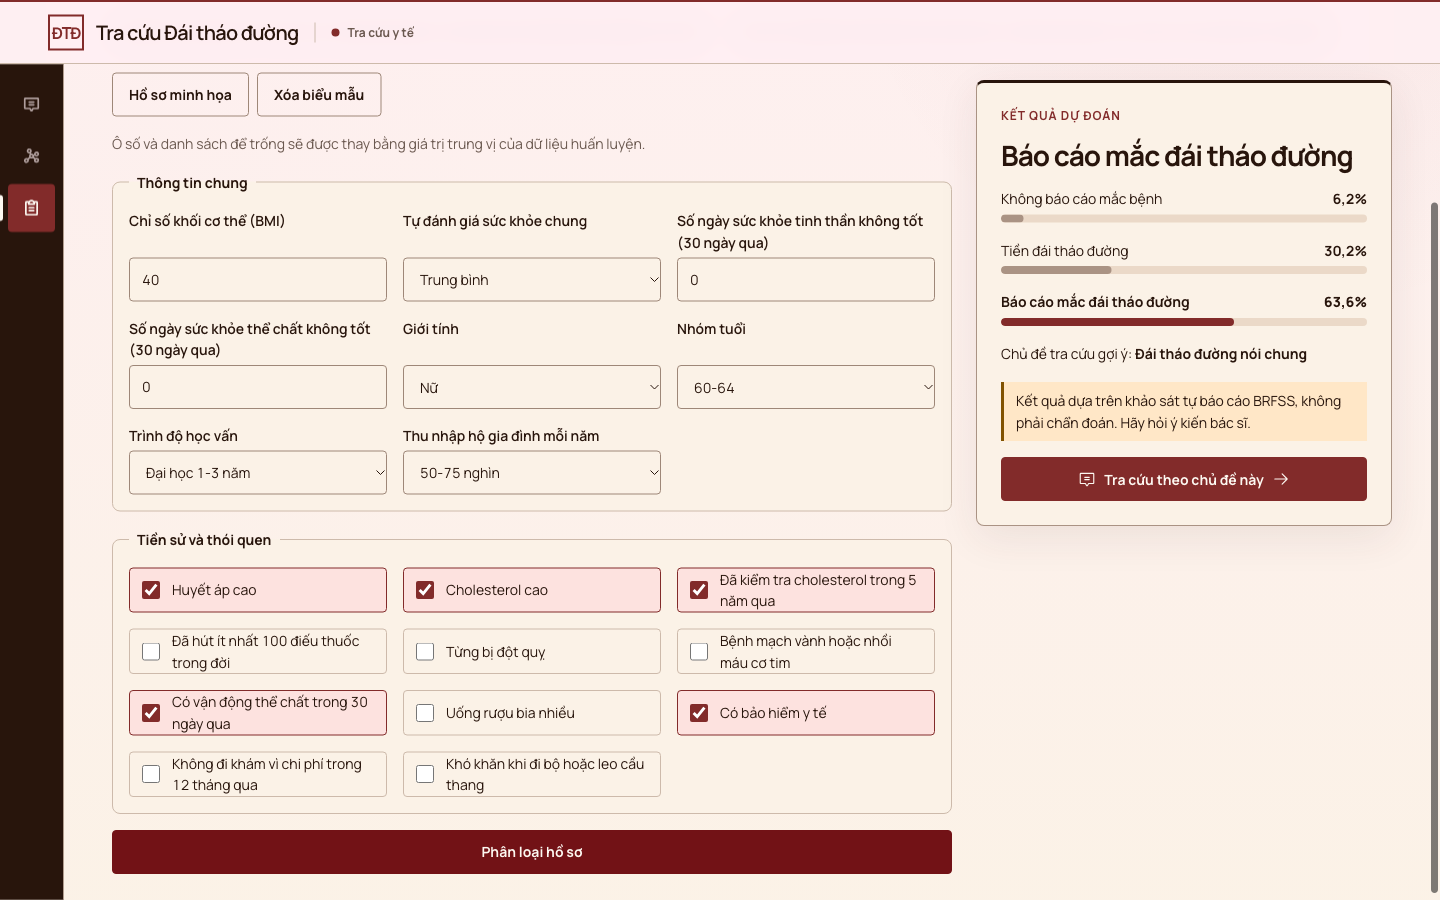
\includegraphics[width=0.49\linewidth]{../results/screens/u7b/classify.png}\hfill
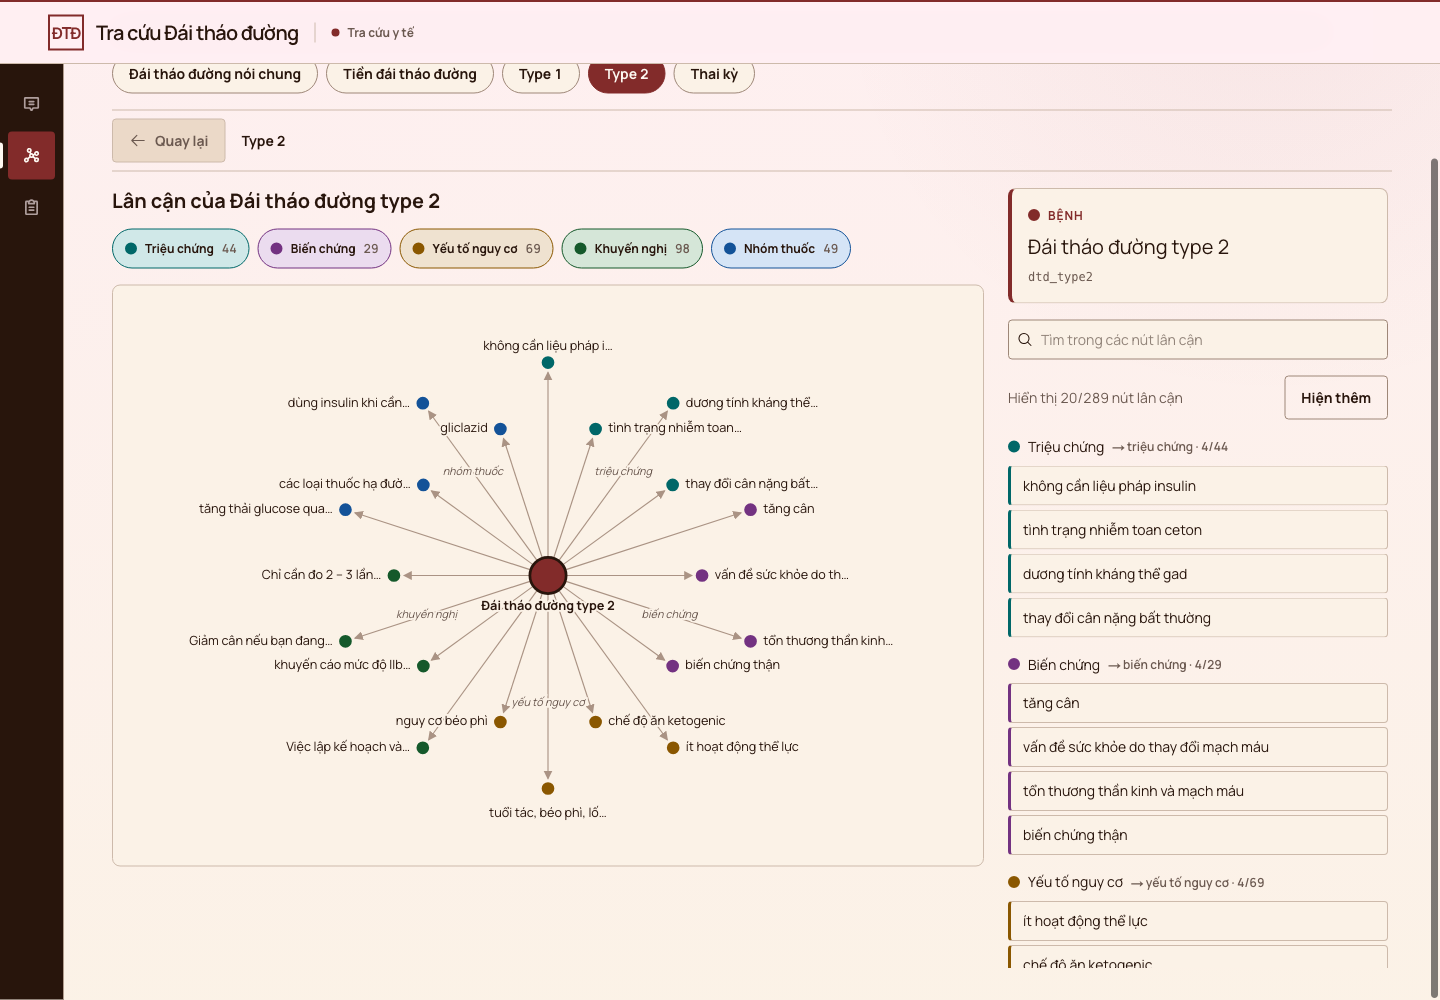
\includegraphics[width=0.49\linewidth]{../results/screens/u7b/graph.png}
\caption{Trang phân loại với hồ sơ minh họa (trái) và trang đồ thị tri thức quanh nút đái tháo đường típ 2 (phải).
Bấm một nút lân cận để đi tiếp tới khuyến nghị, đoạn văn và tài liệu nguồn.}
\end{figure}

Đo trên giao diện bằng trình duyệt tự động, thời gian từ lúc bấm gửi đến khi chữ đầu tiên xuất hiện có trung vị
\uiFirstTextP{} giây trên 5 câu hỏi; phần lớn là thời gian gọi mô hình ngôn ngữ.

\subsection{Giới hạn và hướng phát triển}

\paragraph{Dữ liệu và đánh giá.}
Nhãn khảo sát là tự báo cáo, không có xét nghiệm xác nhận, và các chỉ số chưa dùng trọng số thiết kế của BRFSS nên
chỉ mô tả mẫu, không ước lượng cho dân số. Bộ đánh giá RAG có \nQuestions{} câu và tập tham chiếu do mô hình ngôn ngữ
gán; đọc lại mẫu cho thấy khoảng \relAgree{} nhãn đúng. Một số chênh lệch nhỏ giữa các cấu hình (một câu hỏi) nằm
trong mức dao động của một lần chạy. Hệ thống chưa được chuyên gia y tế đánh giá.

\paragraph{Đồ thị.}
Việc gộp dữ kiện còn yếu do tên ngắn không thống nhất, nên số dữ kiện được hai ngôn ngữ cùng hỗ trợ còn ít. Hướng
tiếp theo là gộp dữ kiện bằng độ gần vector của tên và câu trích, sau đó đo lại đóng góp của bước mở rộng. Phân loại
loại dữ kiện cũng cần một bước kiểm riêng.

\paragraph{Thời gian phản hồi.}
Vì cổng trích dẫn chạy trên toàn bộ câu trả lời, chữ đầu tiên chỉ xuất hiện khi mô hình đã viết xong. Có thể kiểm
từng câu khi mô hình viết tới dấu chấm để hiện chữ sớm hơn mà vẫn giữ nguyên quy tắc không hiện ý chưa qua kiểm tra.

% ==================================================================
\section{Kết luận}

Bài làm dựng được một hệ thống tra cứu đái tháo đường chạy được từ đầu đến cuối: \nDocs{} tài liệu hai ngôn ngữ được
tổ chức thành đồ thị Neo4j, câu trả lời luôn chỉ về đoạn nguồn cụ thể, và hệ thống từ chối khi không có bằng chứng.
Trên bộ kiểm tra, \supportedTwo{} phát biểu được nguồn hỗ trợ và cả \nOos{} câu ngoài phạm vi đều bị từ chối.

Hai kết quả đo đáng chú ý đi ngược kỳ vọng ban đầu. Thứ nhất, xếp hạng chỉ bằng vector tốt hơn mọi cách gộp với BM25
và đồ thị; đồ thị có ích hơn khi dùng để bổ sung ngữ cảnh và bằng chứng ở ngôn ngữ khác. Thứ hai, phần lớn lỗi lớn
trong quá trình làm nằm ở hệ thống đo và ở bước xử lý định dạng trích dẫn, không ở mô hình; cả hai chỉ lộ ra khi đọc
đầu ra thô thay vì tin con số tổng hợp.

Bộ phân loại khảo sát nhận diện kém các nhóm ít mẫu: lớp tiền đái tháo đường gần như không học được, và dự đoán Type 1
có tỷ lệ báo động sai cao. Nhãn dự đoán vì vậy chỉ dùng để gợi ý chủ đề đọc, không dùng để kết luận tình trạng của
một người.

% ==================================================================
\section{Tài liệu tham khảo}
\sloppy

\begin{enumerate}[label={[\arabic*]}]
  \item CDC. Behavioral Risk Factor Surveillance System, 2023 Annual Survey Data. \url{https://www.cdc.gov/brfss/annual_data/annual_2023.html}.
  \item Bộ Y tế. Quyết định 5481/QĐ-BYT ngày 30/12/2020 ban hành tài liệu chuyên môn “Hướng dẫn chẩn đoán và điều trị đái tháo đường típ 2”.
  \item NIDDK. Diabetes overview. \url{https://www.niddk.nih.gov/health-information/diabetes}.
  \item WHO. Diabetes fact sheet. \url{https://www.who.int/news-room/fact-sheets/detail/diabetes}.
  \item Neo4j. Cypher Manual, Vector indexes. \url{https://neo4j.com/docs/cypher-manual/current/indexes/semantic-indexes/vector-indexes/}.
  \item Chen J. và cộng sự. BGE M3-Embedding: Multi-Lingual, Multi-Functionality, Multi-Granularity Text Embeddings. 2024. \url{https://huggingface.co/BAAI/bge-m3}.
  \item Cormack G., Clarke C., Büttcher S. Reciprocal Rank Fusion outperforms Condorcet and individual rank learning methods. SIGIR 2009.
  \item Guo C. và cộng sự. On Calibration of Modern Neural Networks. ICML 2017.
  \item Lewis P. và cộng sự. Retrieval-Augmented Generation for Knowledge-Intensive NLP Tasks. NeurIPS 2020.
\end{enumerate}

Danh sách đầy đủ \nDocs{} tài liệu trong kho tri thức, kèm địa chỉ và ngày tải, nằm trong
\texttt{data/processed/documents.jsonl} và \texttt{pipeline/sources.yaml}.

\end{document}
